\ifdefined\ishandout
\documentclass[handout]{beamer}
\else
\documentclass{beamer}
\fi

\usepackage[frenchb]{babel}
\usepackage[T1]{fontenc}
\usepackage[latin1]{inputenc}
\usepackage{hyperref}
\usepackage{multirow}
\usepackage{listings}
\usepackage{fancyvrb}
\usepackage{tikz}
\usepackage{framed}
\usepackage{algorithm}
\usepackage{algorithmic}
\usepackage{xcolor}
\usepackage{color, colortbl}
\usepackage{handoutWithNotes}

\usetikzlibrary{shapes.geometric}
\usetikzlibrary{positioning}
\usetikzlibrary{shapes.arrows, chains}
\usetikzlibrary{arrows,calc}
\usepackage{array}
\usetheme{Boadilla}

\ifdefined\ishandout
\pgfpagesuselayout{3 on 1 with notes}[a4paper,border shrink=5mm]
\usecolortheme{dove}
\else
\usecolortheme{dolphin}
\fi


\lstnewenvironment{codeC}
{ \lstset{language=C,
    otherkeywords={printf,scanf}}
}
{}

\ifdefined\ishandout
\definecolor{mygreen}{rgb}{0,0,0}
\definecolor{mymauve}{rgb}{0,0,0}
\definecolor{myblue}{rgb}{0,0,0}
\else
\definecolor{mygreen}{rgb}{0,0.6,0}
\definecolor{mymauve}{rgb}{0.58,0,0.82}
\definecolor{myblue}{rgb}{0,0,1}

\fi

\definecolor{mygray}{rgb}{0.5,0.5,0.5}


\lstset{language=C,
% breakatwhitespace=false,         % sets if automatic breaks should only happen at whitespace
%  breaklines=true,                 % sets automatic line breaking
%  captionpos=b,                
commentstyle=\itshape\color{mymauve},
keywordstyle=\bfseries\color{myblue},
%numbers=left,                    % where to put the line-numbers; possible values are (none, left, right)
%  numbersep=8pt,                   % how far the line-numbers are from the code
%  numberstyle=\tiny\color{mygray}, % the style that is used for the line-numbers
  rulecolor=\color{black},         % if not set, the frame-color may be changed on line-breaks within not-black text (e.g. comments (green here))
%  showspaces=false,                % show spaces everywhere adding particular underscores; it overrides 'showstringspaces'
  showstringspaces=false,          % underline spaces within strings only
%  showtabs=false,                  % show tabs within strings adding particular underscores
%  stepnumber=2,                    % the step between two line-numbers. If it's 1, each line will be numbered
  stringstyle=\color{mygreen},     % string literal style
%  tabsize=2 
}

\newcommand{\red}{\textcolor{red}}
%\newcommand \emph
%Default size : 12.8 cm * 9.6 cm

\newcommand{\tmark}[1]{\tikz[remember picture, baseline=-.5ex]{\coordinate(#1)}}

\ifdefined\ishandout
\newenvironment<>{codeblock}[1]{%begin
  \setbeamercolor{block title}{fg=black,bg=lightgray!80}%
  \begin{block}{#1}}
  % \begin{codeC}}
  %  {\end{codeC}
{  
\end{block}}

\newenvironment<>{termblock}[1]{
    \setbeamercolor{block title}{fg=black,bg=lightgray!90}%
    \begin{block}{#1}
}
%     \begin{Verbatim}}
{%\end{Verbatim}
\end{block}
}

\definecolor{bluegreen}{RGB}{0,0,0}
%\definecolor{bluegreen}{rgb}{0,0.6,0.8}
\else

\newenvironment<>{codeblock}[1]{%begin
  \setbeamercolor{block title}{fg=darkgray,bg=yellow}%
  \begin{block}{#1}}
  % \begin{codeC}}
  %  {\end{codeC}
{  
\end{block}}

\newenvironment<>{termblock}[1]{
    \setbeamercolor{block title}{fg=white,bg=lightgray}%
    \begin{block}{#1}}
%     \begin{Verbatim}}
{%\end{Verbatim}
\end{block}
}

\definecolor{bluegreen}{RGB}{0,149,182}
%\definecolor{bluegreen}{rgb}{0,0.6,0.8}
\fi

%\newcommand{\output}[1]{
\setbeamertemplate{navigation symbols}{}
\newcommand{\bvrb}{\Verb[commandchars=���,formatcom=\color{bluegreen}]}
\newcommand{\footvrb}{\footnotesize\Verb}


%%% Param�tres du cours (� r�gler)
%Num�ro du cours
\newcommand{\nb}{4}

\title[Cours n�\nb]{Cours n�\nb - Inputs/Ouptut\\Les Fonctions}
\author[]{julien.brajard@upmc.fr}
\institute[Polytech' UPMC]{Polytech' UPMC}
\date{10 Octobre 2016}
\begin{document}
%%%%%%%%%%%%%%%%%%%%% SLIDES DE TITRE
\begin{frame}
\titlepage
\centering{
\url{http://australe.upmc.fr} (onglet EPU-C5-IGE Info Gen)}
\end{frame}
%%%%%%%%%%%%%%%%%%%%%
\begin{frame}
\frametitle{Plan du cours n�\nb}
\tableofcontents[hideallsubsections]
\end{frame}

%%%%



%%%%%% SECTION 12
% !TEX encoding = IsoLatin9

%%%%%%%%%%%%%%%%%%%%% SECTION 1
\section{Entr�es/Sorties}
\begin{frame}
  \begin{columns}
    \column{4.8cm}
    \tableofcontents[currentsection,hideothersubsections]
    \column{7cm}
     \centering{
      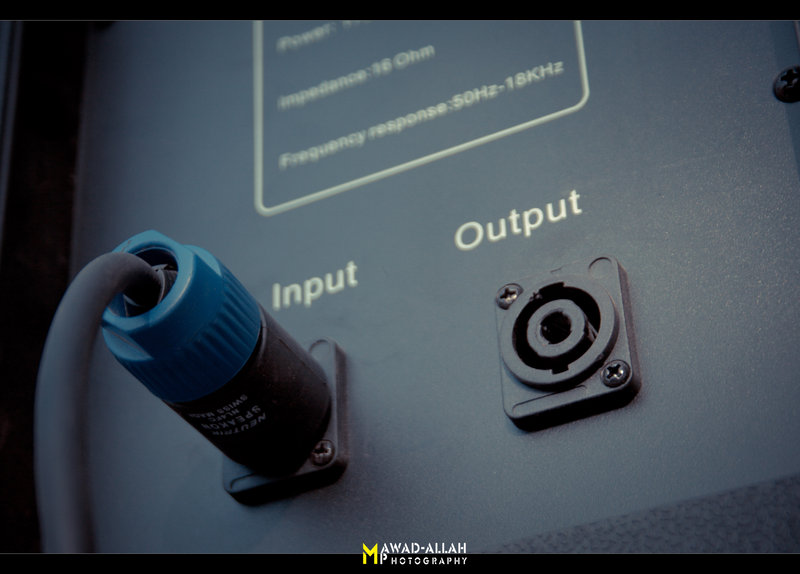
\includegraphics[width=5cm]{fig/inout.jpg}
}
  \end{columns}
  
\end{frame}

\begin{frame}[fragile]
\frametitle{Les entr�es/sorties}
\begin{itemize}
\item Affichage de caract�res � l'�cran : \\
\bvrb|printf(�textit�chaine_de_caracteres�,�textit�variables�);|\\
\vspace{0.5cm}
\item Lecture de caract�res au clavier : \\
\bvrb|scanf(�textit�format�,�textit�adresses�);|\\
\vspace{0.5cm}
\item Pour utiliser ces fonctions, il est n�cessaire d'inclure au programme
la biblioth�que \Verb|stdio.h| g�rant les entr�es sorties :
\begin{codeblock}{}
\lstset{escapeinside={��}}
%\lstset{basicstyle=\scriptsize}
\begin{codeC}
#include <stdio.h>
\end{codeC}
\end{codeblock}

\end{itemize}
\end{frame}

\begin{frame}[fragile]
\frametitle{Comment fonctionne le \bvrb|scanf| ?}
\begin{figure}
\centering
\begin{tikzpicture} [
  auto,
  line/.style     = { draw, thick, color=red,->, shorten >=2pt },
  node distance = 4cm
]
\node[inner sep=0pt] (clavier)
{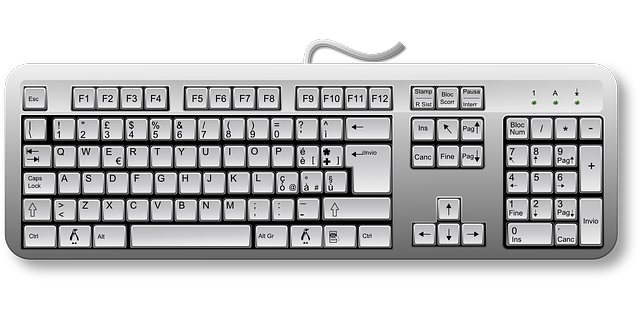
\includegraphics[width=3cm]{./fig/clavier.png}};
\node[inner sep=0pt,right of=clavier] (fils) 
{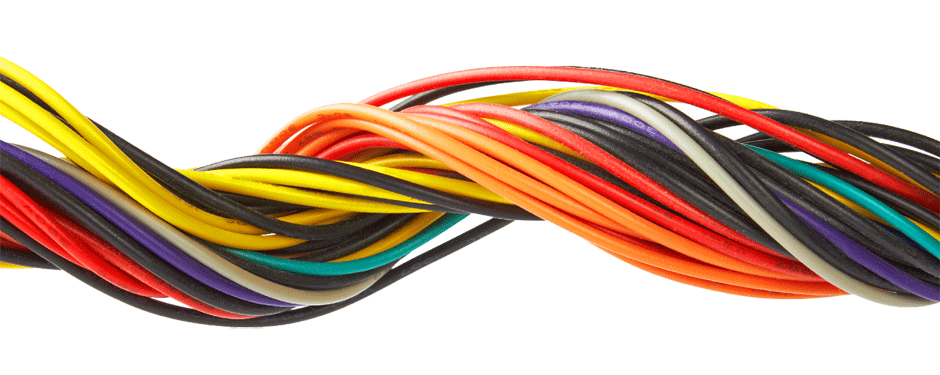
\includegraphics[width=3cm]{./fig/cables.png}};
\node[inner sep=0pt,right of=fils] (proc) 
{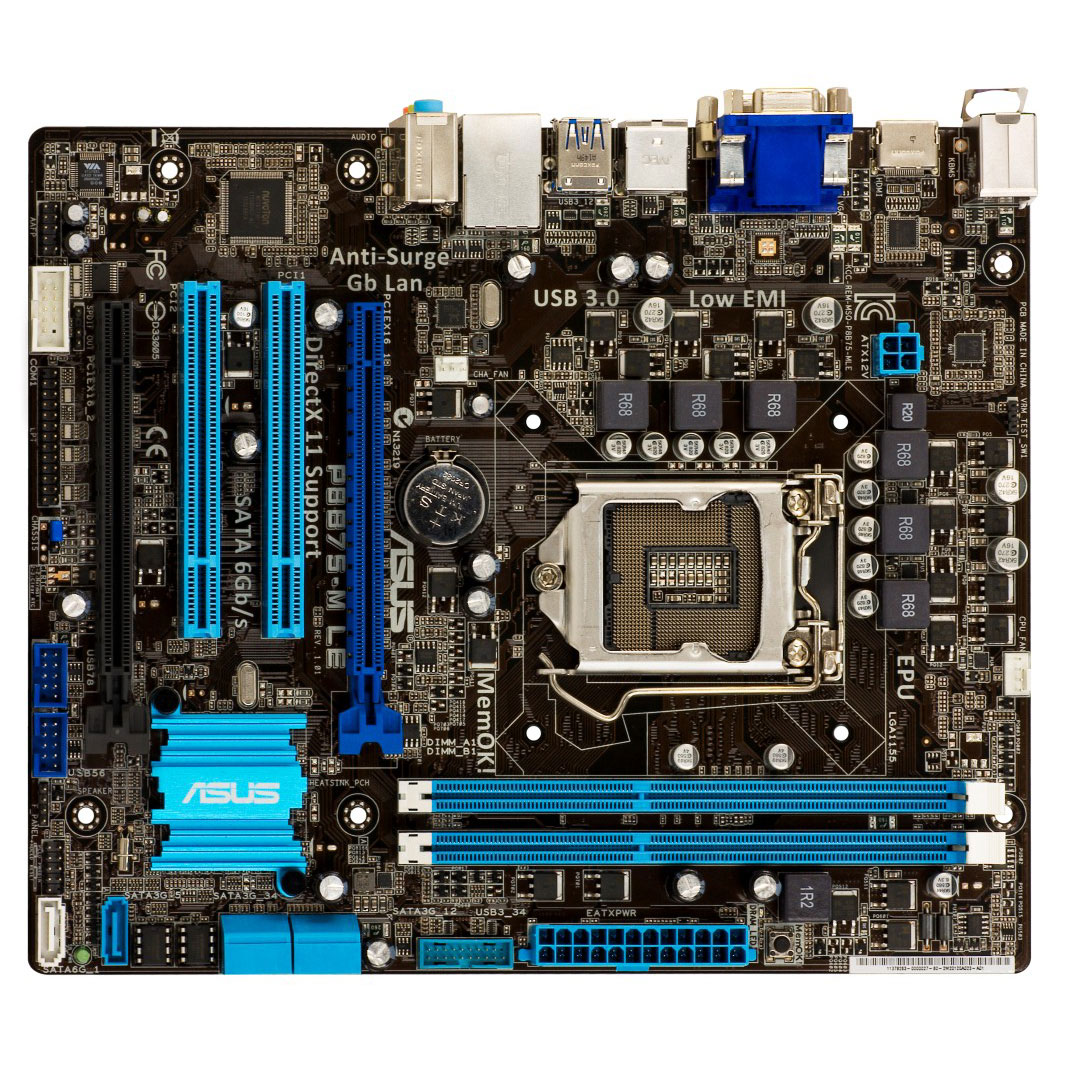
\includegraphics[width=3cm]{./fig/carte_mere.jpg}};
\node [below of = clavier,yshift = +2cm] (input) {{\Large 5}};
\node [below of = proc, yshift  = +2cm] (mem)
{
  \begin{tabular}{p{0.9em}|p{0.9em}|p{0.9em}|p{0.9em}|p{0.9em}}
    \hline
    ... & & 5 & & ... \\
    \hline
    \multicolumn{2}{p{1.8em}}{} &\multicolumn{1}{p{0.9em}}{\texttt{\&n}} & \multicolumn{2}{p{1.8em}}{}  \\
  \end{tabular}
};
\path [line] (input) -- (mem);
\end{tikzpicture}
\end{figure}

\begin{columns}
\column{0.45\textwidth}
\begin{codeblock}{}
\lstset{escapeinside={��}}
%\lstset{basicstyle=\scriptsize}
\begin{codeC}
scanf("%d",&n);
\end{codeC}
\end{codeblock}
\column{0.45\textwidth}
La valeur 5 est affect�e � la variable \Verb|n|.

La case m�moire adress�e par \Verb|&n| contient la 
valeur 5
\end{columns}


\end{frame}


\begin{frame}[fragile]
\frametitle{Comment fonctionne le \bvrb|printf| ?}
\begin{figure}
\centering
\begin{tikzpicture} [
  auto,
  line/.style     = { draw, color=red, thick, ->, shorten >=2pt },
  node distance = 4cm
]
\node[inner sep=0pt] (proc) 
{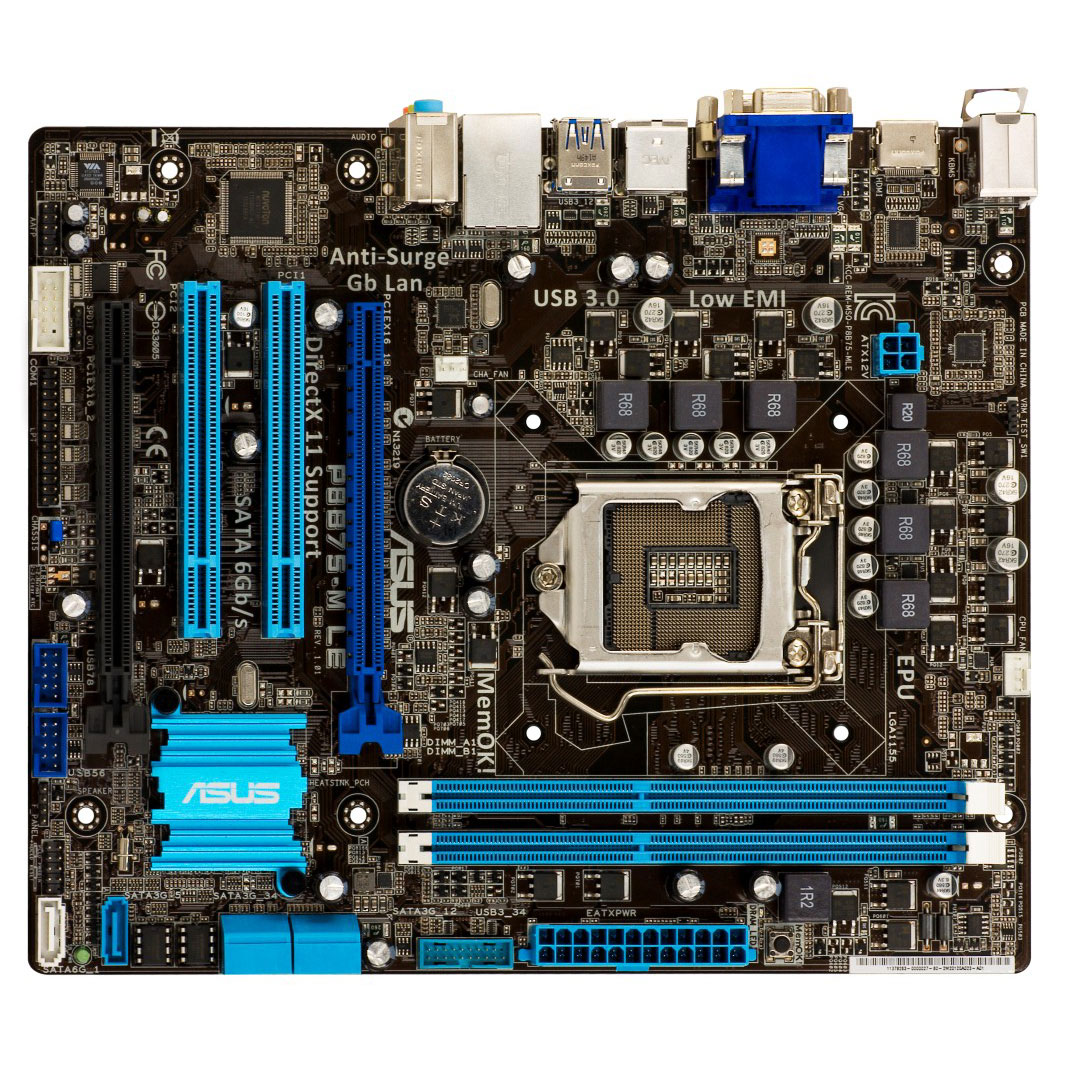
\includegraphics[width=3cm]{./fig/carte_mere.jpg}};
\node[inner sep=0pt,right of=proc] (fils) 
{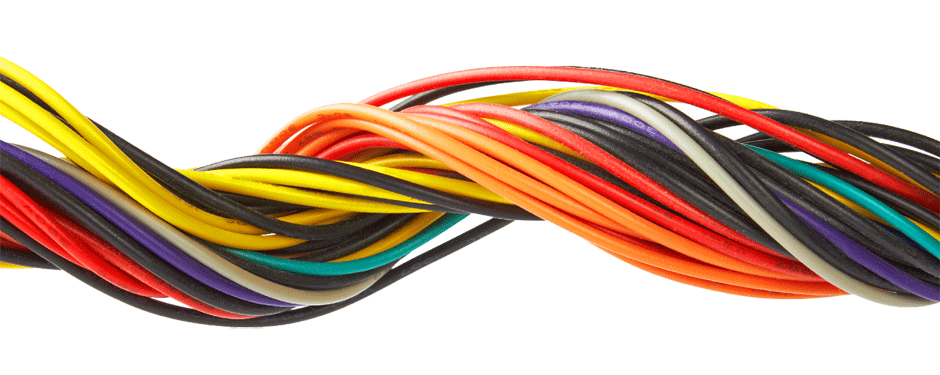
\includegraphics[width=3cm]{./fig/cables.png}};
\node[inner sep=0pt, right of=fils] (ecran)
{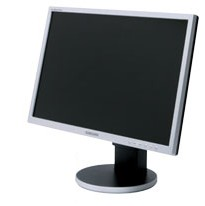
\includegraphics[width=3cm]{./fig/ecran.jpg}};

\node [below of = ecran,yshift = +2cm] (output) {{\Large 5}};
\node [below of = proc, yshift  = +2cm] (mem)
{
  \begin{tabular}{p{0.9em}|p{0.9em}|p{0.9em}|p{0.9em}|p{0.9em}}
    \hline
    ... & & 5 & & ... \\
    \hline
    \multicolumn{2}{p{1.8em}}{} &\multicolumn{1}{p{0.9em}}{\texttt{\&n}} & \multicolumn{2}{p{1.8em}}{}  \\
  \end{tabular}
};
\path [line] (mem) -- (output);
\end{tikzpicture}
\end{figure}

\begin{columns}
\column{0.45\textwidth}
\begin{codeblock}{}
\lstset{escapeinside={��}}
%\lstset{basicstyle=\scriptsize}
\begin{codeC}
printf("%d",n);
\end{codeC}
\end{codeblock}
\column{0.45\textwidth}
Affiche la valeur de la variable \Verb|n|.

La case m�moire adress�e par \Verb|&n| est affich�.
\end{columns}


\end{frame}

\begin{frame}[fragile]
\frametitle{Les codes formats}
\begin{table}
\begin{tabular}{|l|l|}
\hline
\bvrb|%c| & Caract�re \\
\hline
\bvrb|%d| & Entier sign� \\
\hline
\bvrb|%u| & Entier non sign� \\
\hline
\bvrb|%x| ou \bvrb|%X| & Entier en hexad�cimal \\
\hline
\bvrb|%o| & Entier en octal\\
\hline
\bvrb|%ld| & Entier long sign� \\
\hline
\bvrb|%lu| & Entier long non sign� \\
\hline
\bvrb|%lx| ou \bvrb|%lX| & Entier long en hexad�cimal \\
\hline
\bvrb|%f| & R�el simple pr�cision avec virgule flottante \\
\hline
\bvrb|%e| ou \bvrb|%E| & R�el simple pr�cision avec exposant e ou E \\
\hline
\bvrb|%lf| & R�el double avec virgule flottante \\
\hline
\bvrb|%le| ou \bvrb|%lE| & R�el double avec exposant e ou E \\
\hline
\bvrb|%Lf| & R�el long double avec virgule flottante \\
\hline
\bvrb|%Le| ou \bvrb|%LE| & R�el long double avec exposant e ou E \\
\hline
\bvrb|%s| & Cha�ne de caract�res \\
\hline
\bvrb|%p| & Pointeur \\
\hline
\end{tabular}
\end{table}

\end{frame}

\begin{frame}[fragile]
\frametitle{Compl�ments sur les formats}

\begin{itemize}
\item Autres formats d'affichage :\\
\begin{description}
\item[]\bvrb|\n| : Passage � la ligne.\\
\item[]\bvrb|\t| : Tabulation.\\
\item[]\bvrb|\0| : Fin de cha�ne.\\
\item[]\bvrb|\%| : Signe pourcentage.\\
\end{description}
\item On peut pr�c�der les codes des r�els de deux entiers : \bvrb|%n.p|
\begin{description}
\item[]\bvrb|n| : largeur minimale \\
\item[]\bvrb|p| : pr�cisions \\
\end{description}
\item On peut pr�c�der les codes des entiers d'un entier :
\begin{description}
\item[]\bvrb|%n| : largeur minimale de n.\\
\item[]\bvrb|%0n| : largeur minimal de n avec les blancs combl�s par des z�ros.\\
\end{description}

\end{itemize}

\end{frame}

\begin{frame}[fragile]
\frametitle{Exemples}

\begin{codeblock}{}
\lstset{escapeinside={��}}
%\lstset{basicstyle=\scriptsize}
\begin{codeC}
 int n=34 ;
 float x = 3.1,y=1.525;
 printf("_%d_%3d_%1d_%03d_\n",n,n,n,n);
 printf("_%f_%3.2f_\n",x,x);
 printf("_%f_%5.2f_%2.2f_\n",y,y,y);
\end{codeC}
\end{codeblock}
\begin{termblock}{Test d'ex�cution}
\lstset{escapeinside={��}}
\begin{Verbatim}
_34_ 34_34_034_
_3.100000_3.10_
_1.525000_ 1.52_1.52_
\end{Verbatim}
\end{termblock}


\end{frame}

\begin{frame}[fragile]
\frametitle{\bvrb|scanf| : comment �a se passe ?}
\begin{codeblock}{}
\vspace{-0.2cm}
\lstset{escapeinside={��}}
%\lstset{basicstyle=\scriptsize}
\begin{codeC}
int a; float x ;
scanf("%d %f",&a,&x);
\end{codeC}
\vspace{-0.2cm}
\end{codeblock}
\begin{enumerate}[<+->]
\item Si le tampon est vide, le programme s'interrompt pour laisser
l'utilisateur taper au clavier.\\
\item D�s que la touche \Verb|Entr�e| est frapp�e, la s�quence des �lements
entr�s est stock�e dans une zone m�moire appel�e \red{tampon}.\\
\item La directive \bvrb|scanf| consomme la m�moire tampon en fonction
du format indiqu� et stocke les �l�ments convertis dans les variables :\\
\begin{itemize}
\item Si le tampon est vide avant que le format du \bvrb|scanf| ne soit
enti�rement converti, on retourne � l'�tape 1.\\
\item Si le format dans le \bvrb|scanf| ne correspond pas au prochain caract�re de la s�quence
entr�e au clavier, \red{la conversion s'interrompt et le programme continue}.\\
\item Si la conversion est enti�rement termin�e, le programme continue
mais \red{il peut rester encore des �l�ments dans le tampon}.\\
\end{itemize}
\end{enumerate}

\end{frame}

\begin{frame}[t,fragile]
\frametitle{Illustration}
\begin{columns}[t]
\column{0.4\textwidth}
\begin{codeblock}{}
\vspace{-0.2cm}
\lstset{escapeinside={��}}
%\lstset{basicstyle=\scriptsize}
\begin{codeC}
int a; float x ;
scanf("%d %f",&a,&x);�\tikz[remember picture,baseline=-.5ex]\coordinate(code);�
\end{codeC}
\vspace{-0.2cm}
\end{codeblock}
\vspace{0.5cm}
\begin{visibleenv}<3->
\begin{termblock}{au clavier : \tikz[remember picture,baseline=-.5ex]\coordinate(clav);   }
\lstset{escapeinside={��}}
\begin{lstlisting}
3 2.5 (Entr�e)�\tikz[remember picture,baseline=-.5ex]\coordinate(term);�
\end{lstlisting}
\end{termblock}
\vspace{0.4cm}
\end{visibleenv}

\begin{visibleenv}<6->

L'espace est ignor� \tikz[remember picture,baseline=-.5ex]\coordinate(space);\\
\red{sauf} si le format \bvrb|%c|
(caract�re) est sp�cifi�.
\end{visibleenv}

\column{0.55\textwidth}
\vspace{-0.5cm}
\begin{figure}
  % \centering
  \begin{tikzpicture}[
    auto,
    remember picture,
    node distance = 2cm,
    fond/.style = {rectangle,draw=blue!80, rectangle, minimum width=5.5cm, minimum height = 1.5cm, fill=blue!20},
    head/.style={regular polygon, xshift=-2.27cm,yshift=0.13cm,fill=black,rotate around = {60:(0,0)},regular polygon sides = 3, inner sep=0.05cm},
    ]
    \node <2->(boite1) [fond]{};
    \node <4->(boite2) [fond,below of = boite1]{};
    \node <5->(boite3) [fond,below of = boite2]{};
    \node <7->(boite4) [fond,below of = boite3]{};
    
    \node <2->(tampon1)
    {
      \begin{tabular}{|p{0.35cm}|p{0.35cm}|p{0.35cm}|p{0.35cm}|p{0.1cm}|p{0.35cm}|p{0.35cm}|}
        \multicolumn{4}{c}{tampon}& \multicolumn{1}{c}{} & \multicolumn{1}{c}{\texttt{\&a}} & \multicolumn{1}{c}{\texttt{\&x}} \\
        \cline{1-4}\cline{6-7}
        & & & & & & \\
        \cline{1-4}\cline{6-7}
      \end{tabular}
    };
    \node <2-> (tik1) [head] {};
    
    \node <4-> (tampon2) [below of = boite1]
    {
      \begin{tabular}{|p{0.35cm}|p{0.35cm}|p{0.35cm}|p{0.35cm}|p{0.1cm}|p{0.35cm}|p{0.35cm}|}
        \multicolumn{4}{c}{tampon}& \multicolumn{1}{c}{} & \multicolumn{1}{c}{\texttt{\&a}} & \multicolumn{1}{c}{\texttt{\&x}} \\
        \cline{1-4}\cline{6-7}
        \footvrb|3| & & \footvrb|2.5| & \footvrb|\n| & & & \\
        \cline{1-4}\cline{6-7}
      \end{tabular}
    };

\node <4->(tik2) [below of =boite1, head] {};
        \node  <5-> (tampon3) [below of = boite2]
    {
      \begin{tabular}{|p{0.35cm}|p{0.35cm}|p{0.35cm}|p{0.35cm}|p{0.1cm}|p{0.35cm}|p{0.35cm}|}
        \multicolumn{4}{c}{tampon}& \multicolumn{1}{c}{} & \multicolumn{1}{c}{\texttt{\&a}} & \multicolumn{1}{c}{\texttt{\&x}} \\
        \cline{1-4}\cline{6-7}
        & \footvrb|2.5| & \footvrb|\n| & & & 3 & \\
        \cline{1-4}\cline{6-7}
      \end{tabular}
    };
    \node <5->(tik3) [below of =boite2, head] {};
    \node <7->(tampon4) [below of = boite3]
    {
      \begin{tabular}{|p{0.35cm}|p{0.35cm}|p{0.35cm}|p{0.35cm}|p{0.1cm}|p{0.35cm}|p{0.35cm}|}
        \multicolumn{4}{c}{tampon}& \multicolumn{1}{c}{} & \multicolumn{1}{c}{\texttt{\&a}} & \multicolumn{1}{c}{\texttt{\&x}} \\
        \cline{1-4}\cline{6-7}
        \footvrb|\n| & & & & & 3 & 2.5 \\
        \cline{1-4}\cline{6-7}
      \end{tabular}
    };
    \node <7->(tik4) [below of =boite3, head] {};
  \end{tikzpicture}
\end{figure}

\begin{tikzpicture}[
  remember picture,
  overlay,
  line/.style= {draw=red, very thick, ->},
  ]
  \draw <2-> [line] ($(code)+(0,0)$) -- ($(tampon1.west)+(0,-0.2)$) ;
  \draw<3-> [line] ($(tampon1.west)+(0,-0.6)$) -- ($(clav)+(0,0)$) ;
\draw <4-> [line] ($(term)+(0,0)$) -- ($(tampon2.west)+(0,-0.2)$) ;
  \draw<5-> [line] ($(tampon2.west)+(0.5,-0.4)$) -- ($(tampon3.east)+(-1.6,+0.1)$) node[midway,above,sloped]{\red{\texttt{\%d}}};
  \draw<7-> [line] ($(tampon3.west)+(1.5,-0.4)$) -- ($(tampon4.east)+(-0.6,+0.1)$) node[midway,above,sloped]{\red{\texttt{\%f}}};
  \draw<6-> [->] ($(tampon3.west)+(0,-0.2)$) -- (space) ;

\end{tikzpicture}

\end{columns}

\end{frame}

\begin{frame}[fragile]
\frametitle{Faire attention}
\begin{itemize}
\item Les caract�res peuvent rester dans le tampon (Exemple~1).\\
\vspace{0.4cm}
\item Le caract�re espace est pris en compte seulement dans le cas
du formateur \bvrb|%c| (Exemple~2).\\
\vspace{0.4cm}
\item La conversion peut s'arr�ter et ainsi des variables peuvent ne pas
�tre attribu�es (Exemple~3).\\
\end{itemize}
\end{frame}

\begin{frame}[t,fragile]
\frametitle{\label{exemple1} Exemple 1}
\begin{codeblock}{}
\vspace{-0.2cm}
\lstset{escapeinside={��}}
%\lstset{basicstyle=\scriptsize}
\begin{codeC}
int a; float x ;
printf("Ecrire a : ");
scanf("%d",&a);
printf("Ecrire x :");
scanf("%f",&x);
printf("Fin\n");
\end{codeC}
\vspace{-0.2cm}
\end{codeblock}
\vspace{-0.5cm}
\begin{columns}[t]
\column{0.48\textwidth}
\begin{termblock}{Test d'ex�cution}
\lstset{escapeinside={��}}
\begin{Verbatim}
Ecrire a : 32 (Entr�e)
Ecrire x : 2.1 (Entr�e)
Fin
\end{Verbatim}
\end{termblock}
Ce fonctionnement est normal :
Le 1er \bvrb|scanf| consomme l'entier \verb|32|
et le 2�me consomme le r�el \verb|2.1|.

\column{0.48\textwidth}
\begin{termblock}{Test d'ex�cution}
\lstset{escapeinside={��}}
\begin{Verbatim}
Ecrire a : 3 2 (Entr�e)
Ecrire x : 
Fin
\end{Verbatim}
\end{termblock}
On a s�par� (par erreur) le 3 et le 2.
Le premier \bvrb|scanf| consomme
le 3. Le deuxi�me \bvrb|scanf| consomme le 2 sans redonner la main
� l'utilisateur.
\end{columns}

\end{frame}

\begin{frame}[fragile]
\frametitle{Solution}
On peut �crire une petite proc�dure qui vide le tampon apr�s chaque scanf.
\begin{codeblock}{}
\vspace{-0.2cm}
\lstset{escapeinside={��}}
%\lstset{basicstyle=\scriptsize}
\begin{codeC}
int a ; float x ;
char c;
printf("Ecrire a : ");
scanf("%d",&a);
do {
  c = getchar();
  } while (c!='\n' && c!=EOF);
printf("Ecrire x : ";
scanf("%f",&x);
\end{codeC}
\vspace{-0.2cm}
\end{codeblock}

\vspace{0.2cm}

\bvrb|getchar| lit un caract�re \Verb|c| dans le tampon
tant que (\bvrb|while|) \Verb|c| est diff�rent de \Verb|\n| ou
\Verb|EOF| (fin du tampon).

\end{frame}

\begin{frame}[t,fragile]
\frametitle{\label{exemple2} Exemple 2}
\begin{codeblock}{}
\vspace{-0.2cm}
\lstset{escapeinside={��}}
%\lstset{basicstyle=\scriptsize}
\begin{codeC}
char c;
scanf("%c",&c);
\end{codeC}
\vspace{-0.2cm}
\end{codeblock}


\centering{
un espace\\
\tikz[remember picture,baseline=-.5ex]\coordinate(sp1);
}
\vspace{-0.5cm}


\begin{columns}[t]
\column{0.48\textwidth}
\begin{termblock}{Test d'ex�cution}
\lstset{escapeinside={��}}
\begin{lstlisting}
A (Entr�e)
\end{lstlisting}
\end{termblock}

La variable \verb|c| contient \verb|'A'|.

\column{0.48\textwidth}
\begin{termblock}{Test d'ex�cution}
\lstset{escapeinside={��}}
\begin{lstlisting}
�\tikz[remember picture,baseline=-.5ex]\coordinate(sp2);� A (Entr�e)
\end{lstlisting}
\end{termblock}
La variable \verb|c| contient \verb|' '|.

\end{columns}

\begin{tikzpicture}[auto, remember picture, overlay]
\draw[thick,->, shorten >= 3pt] (sp1) -- (sp2) ;
\end{tikzpicture}
\end{frame}

\begin{frame}[t,fragile]
\frametitle{Solution}
\begin{codeblock}{}
\vspace{-0.2cm}
\lstset{escapeinside={��}}
%\lstset{basicstyle=\scriptsize}
\begin{codeC}
char c;
scanf("�\tikz[remember picture,baseline=-.5ex]\coordinate(spc1);� %c",&c);
\end{codeC}
\vspace{-0.2cm}
\end{codeblock}
\tikz[remember picture,baseline=-.5ex]\coordinate(spc2);
L'espace indique qu'on ignore les espaces avant le caract�re\\
\vspace{0.5cm}
\centering{
un espace\\
\tikz[remember picture,baseline=-.5ex]\coordinate(sp1);
}
\vspace{-0.5cm}


\begin{columns}[t]
\column{0.48\textwidth}
\begin{termblock}{Test d'ex�cution}
\lstset{escapeinside={��}}
\begin{lstlisting}
A (Entr�e)
\end{lstlisting}
\end{termblock}

La variable \verb|c| contient \verb|'A'|.

\column{0.48\textwidth}
\begin{termblock}{Test d'ex�cution}
\lstset{escapeinside={��}}
\begin{lstlisting}
�\tikz[remember picture,baseline=-.5ex]\coordinate(sp2);� A (Entr�e)
\end{lstlisting}
\end{termblock}
La variable \verb|c| contient \verb|'A'|.

\end{columns}

\begin{tikzpicture}[auto, remember picture, overlay]
\draw[thick,->, shorten >= 3pt] (sp1) -- (sp2) ;
\draw[thick,->, shorten >= 13pt] (spc1) -- (spc2) ;

\end{tikzpicture}
\end{frame}

\begin{frame}[fragile]
\frametitle{Exemple 3}
\begin{codeblock}{}
\vspace{-0.2cm}
\lstset{escapeinside={��}}
%\lstset{basicstyle=\scriptsize}
\begin{codeC}
int a ; float x ;
scanf("%d %f",&a,&x);
\end{codeC}
\vspace{-0.2cm}
\end{codeblock}


\begin{termblock}{Test d'ex�cution}
\lstset{escapeinside={��}}
\begin{lstlisting}
3 k (Entr�e)
\end{lstlisting}
\end{termblock}

La variable \verb|a| a bien �t� initialis�e � 3, mais la variable
\verb|x| n'a pas �t� initialis�e (impossible de convertir \verb|k| en
\bvrb|float|).

\end{frame}

\begin{frame}[fragile]
\frametitle{Solution}
\begin{codeblock}{}
\vspace{-0.2cm}
\lstset{escapeinside={��}}
%\lstset{basicstyle=\scriptsize}
\begin{codeC}
int a ; float x ;
int status ;
status = scanf("%d %f",&a,&x);
if (status != 2)
  {...
\end{codeC}
\vspace{-0.2cm}
\end{codeblock}


\begin{termblock}{Test d'ex�cution}
\lstset{escapeinside={��}}
\begin{lstlisting}
3 k (Entr�e)
\end{lstlisting}
\end{termblock}

La variable \verb|status| sera �gale � 1 (et non comme attendu
� 2). On peut donc pr�voir un traitement sp�cifique � l'aide
d'une structure \bvrb|if|.
\end{frame}




% !TEX encoding = IsoLatin9

%%%�%%%%%%%%%%%%%%%%%% SECTION 1
\section{Les fonctions}
\begin{frame}
  \begin{columns}
    \column{4.8cm}
    \tableofcontents[currentsection,hideothersubsections]
    \column{7cm}
    
  \end{columns}
  
\end{frame}


\begin{frame}
\frametitle{Introduction}
\begin{itemize}
\setlength\itemsep{1em}
\item La r�solution d'un probl�me informatique
peut conduire � la r�solution de plusieurs probl�mes
plus �l�mentaires.
\begin{itemize}
\item Exemple des traitements des tableaux
\end{itemize}
\item Id�e :
\begin{itemize}
\item Identifier ces traitements �l�mentaires 
pour la r�solution du probl�me initial.
\item Construire des petits programmes pour chacun
des traitements �l�mentaires (et les \red{tester}).
\item Ecrire un programme final simple qui utilise
les programmes �l�mentaires comme des briques de base.
\end{itemize}
\end{itemize}
\end{frame}

\begin{frame}
\frametitle{Solution : les fonctions}
\begin{block}{}
Le langage C permet ce d�coupage.
C'est la programmation modulaire.
\end{block}
\begin{itemize}
\item Permet de d�couper un traitement en autant
de traitements �l�mentaires qu'on le souhaite.
\item Permet d'appeler des modules existants (biblioth�que).
\item Permet de d�finir ses modules et de construire ses propres
biblioth�ques.
\item Permet de d�couper un gros logiciel pour faciliter sa mise au point.
\item Evite des copier-coller de code et am�liore sa visibilit�.
\item Permet le travail collaboratif.
\end{itemize}
\end{frame}

\begin{frame}[fragile]
\frametitle{Qu'est-ce qu'une fonction ?}
\begin{alertblock}{}
Une fonction est sous-programme pouvant �tre
appel� dans un programme et qui effectue une 
suite d'op�rations.

Les op�rations effectu�es peuvent d�pendre
de 1 ou plusieurs entr�es et la fonction peut 
renvoyer \red{au plus} une seule sortie (en langage C).
\end{alertblock}
\vspace{1cm}
\begin{figure}
\centering
\begin{tikzpicture} [
       auto,
       function/.style={diamond, draw=blue,thick,fill=blue!20,
               text width = 2cm, text badly centered, rounded corners,
               aspect=2},
       texte/.style={text width = 2cm,text badly centered},
        line/.style     = { draw, thick, ->, shorten >=2pt },
       node distance=4cm,
       ]
       \node (input) [texte]{Entiers, tableaux, r�els, ...};
       \node (fonc) [function, right of = input] {La fonction};
       \node (output) [texte, right of = fonc] {\textbf{Un} entier ou \textbf{Un} r�el, ou ...};
        \begin{scope}[every path/.style=line]
        \path (input) -- (fonc) ;
        \path (fonc) -- (output); 
\end{scope}
\end{tikzpicture}
\end{figure}
\end{frame}

\begin{frame}[fragile]
\frametitle<1>{Exemple : la fonction max}
\frametitle<2>{Terminologie}

\visible<2>{\red{\textbf{D�claration : }}}
\begin{figure}
\centering
\begin{tikzpicture} [
       auto,
       function/.style={diamond, draw=blue,thick,fill=blue!20,
               text width = 2cm, text badly centered, rounded corners,
               aspect=2},
       texte/.style={text width = 2cm,text badly centered},
        line/.style     = { draw, thick, ->, shorten >=2pt },
       node distance=4cm,
       ]
       \node (input) [texte]{Un entier \textbf{a}, Un entier \textbf{b}};
       \node (fonc) [function, right of = input] {max};
       \node (output) [texte, right of = fonc] {\textbf{Un entier} (maximum entre a et b)};
        \begin{scope}[every path/.style=line]
        \path (input) -- (fonc) ;
        \path (fonc) -- (output); 
\end{scope}
\end{tikzpicture}
\end{figure}

\visible<2>{\red{\textbf{Appel : }}}
\begin{figure}
\centering
\begin{tikzpicture} [
       auto,
       function/.style={diamond, draw=blue,thick,fill=blue!20,
               text width = 2cm, text badly centered, rounded corners,
               aspect=2},
       texte/.style={text width = 2cm,text badly centered},
        line/.style     = { draw, thick, ->, shorten >=2pt },
       node distance=4cm,
       ]
       \node (input) [texte]{2\\3};
       \node (fonc) [function, right of = input] {max};
       \node (output) [texte, right of = fonc] {3};
        \begin{scope}[every path/.style=line]
        \path (input) -- (fonc) ;
        \path (fonc) -- (output); 
\end{scope}
\end{tikzpicture}
\end{figure}

\visible<2>{\red{\textbf{D�finition : }}}
\begin{figure}
\centering
\begin{tikzpicture} [
       auto,
       function/.style={diamond, draw=blue,thick,fill=blue!20,
               text width = 2cm, text badly centered, rounded corners,
               aspect=2},
       texte/.style={text width = 2cm,text badly centered},
        line/.style     = { draw, thick, ->, shorten >=2pt },
       node distance=4cm,
       ]
       \node (input) [texte]{Un entier \textbf{a}, Un entier \textbf{b}};
       \node (fonc) [function, right of = input, text width = 3cm, inner sep = 0pt] {{\footnotesize si a<b, renvoyer b\\sinon renvoyer a}};
       \node (output) [texte, right of = fonc] { \textbf{Un entier} (maximum entre a et b)} ;
        \begin{scope}[every path/.style=line]
        \path (input) -- (fonc) ;
        \path (fonc) -- (output); 
\end{scope}
\end{tikzpicture}
\end{figure}
\end{frame}

\begin{frame}[fragile]
\frametitle{En langage C}
\begin{itemize}
\setlength\itemsep{1em}
\item D�claration (le \red{prototype} de la fonction) :\\
\bvrb|�textit�type_retour nom_fonction�(�textit�arguments�);|\\
\item Appel :\\
\bvrb|�textit�nom_fonction�(�textit�liste_valeurs�);|\\
\item D�finition :\\
\bvrb|�textit�type_retour nom_fonction�(�textit�arguments�);|\\
\bvrb|{|\\
\bvrb|�textit�d�claration de variables locales�|\\
\bvrb|�textit�bloc d'instructions�|\\
\bvrb|return �textit�valeur_retour�;|\\
\bvrb|}|
\end{itemize}
\end{frame}

\begin{frame}[fragile]
\frametitle{La fonction \Verb|max|}

\begin{itemize}
\setlength\itemsep{1em}
\item D�claration :\\
\begin{codeblock}{}
\vspace{-.3cm}
\lstset{escapeinside={��}}
\lstset{basicstyle=\scriptsize}
\begin{codeC}
int max (int a, int b);
\end{codeC}
\vspace{-.3cm}
\end{codeblock}

\item Appel :\\
\begin{codeblock}{}
\vspace{-.3cm}
\lstset{escapeinside={��}}
\lstset{basicstyle=\scriptsize}
\begin{codeC}
int maxi ;
int n ;
scanf("%d",&n);
maxi = max(n,3); //Appel de la fonction max
\end{codeC}
\vspace{-.3cm}
\end{codeblock}

\item D�finition :\\
\begin{codeblock}{}
\vspace{-.3cm}
\lstset{escapeinside={��}}
\lstset{basicstyle=\scriptsize}
\begin{codeC}
int max (int a, int b)
{
  if (a<b) return(b) ;
  else return(a) ;
}
\end{codeC}
\vspace{-.3cm}
\end{codeblock}

\end{itemize}
\end{frame}

\begin{frame}[fragile]
\frametitle{Quelque r�gles}
\begin{itemize}
\setlength\itemsep{1em}
\item Une fonction peut �tre d�finie n'importe o� dans le programme ;
\item Une fonction doit �tre d�clar�e avant d'�tre d�clar�e avant d'�tre appel�e pour
la premi�re fois ;
\item Une fonction peut �tre appel�e dans le \bvrb|main| ou dans
une autre fonction ;
\item On ne peut \red{pas} d�finir une fonction dans une autre fonction ;
\item Une fonction peut prendre autant d'argument que l'on souhaite
en entr�e mais ne retour qu'un plus un �l�ment ;
\item Les r�gles sur les noms de fonctions sont les m�mes que
sur les noms de variables.
\end{itemize}
\end{frame}

\begin{frame}[fragile]
\frametitle{Tol�rance}
\begin{block}{}
Si l'on d�finit une fonction avant de l'appeler, on peut �ventuellement
se passer de la d�clarer.
\end{block}
\begin{columns}
\column{.4\textwidth}
\begin{codeblock}{}
\vspace{-.3cm}
\lstset{escapeinside={��}}
\lstset{basicstyle=\scriptsize}
\begin{codeC}
//D�claration-D�finition
int max (int a, int b) {
  if (a<b) return (b) ;
  else return (a) ;
}

//Fonction principale
int main() {
  int maxi, n ;
  scanf("%d",&n);
  maxi = max (n,3);
  printf("%d\n",maxi);
}
\end{codeC}
\vspace{-.3cm}
\end{codeblock}

\column{.15\textwidth}
{\centering {\footnotesize Equivalent
$$\Leftrightarrow$$}}

\column{.4\textwidth}
\begin{codeblock}{}
\vspace{-.3cm}
\lstset{escapeinside={��}}
\lstset{basicstyle=\scriptsize}
\begin{codeC}
//D�claration
int max (int a, int b) ;

//Fonction principale
int main() {
  int maxi, n ;
  scanf("%d",&n);
  maxi = max (n,3);
  printf("%d\n",maxi);
}

//D�finition
int max (int a, int b) {
  if (a<b) return (b) ;
  else return (a) ;
}

\end{codeC}
\vspace{-.3cm}
\end{codeblock}


\end{columns}
\end{frame}

\begin{frame}[fragile]
\frametitle{Fonction appel�e / Fonction appelante}
\begin{columns}
\column{0.45\textwidth}
\begin{codeblock}{}
\vspace{-.3cm}
\lstset{escapeinside={��}}
\lstset{basicstyle=\scriptsize}
\begin{codeC}
//D�claration des fonctions
int f(int a);
int g(int b);

//Fonction principale
int main() {
  int z = 2 ;
  z = g(z) + f(z) ;
  printf("%d\n",z);
 }

//D�finition des fonctions
int f (int a) {
  return (a+2) ;
}

int g (int b) {
  return ( 2*f(b) ) ;
}
\end{codeC}
\vspace{-.3cm}
\end{codeblock}
\column{0.5\textwidth}
\begin{block}{}
Une fonction peut �tre appel�e de n'importe
quelle fonction y compris dans le
\bvrb|main|
\end{block}

\begin{itemize}
\item Fonctions appelantes :
\begin{itemize}
\item \Verb|main| appelle \Verb|g| et \Verb|f|
\item \Verb|g| appelle \Verb|f|
\end{itemize}
\item Fonctions appel�es :
\begin{itemize}
\item \Verb|f| est appel�e par \Verb|main| et \Verb|g|
\item \Verb|g| est appel�e par \Verb|main|
\end{itemize}
\end{itemize}
\end{columns}
\end{frame}
% !TEX encoding = IsoLatin9

%%%%%%%%%%%%%%%%%%%%% SECTION 1
\section{Passage et renvoi de param�tres}
\begin{frame}
  \begin{columns}
    \column{4.8cm}
    \tableofcontents[currentsection,hideothersubsections]
    \column{7cm}
    
  \end{columns}
  
\end{frame}

\begin{frame}[fragile]
\frametitle{Entr�es et sorties}
\begin{block}{Prototype d'une fonction}
\bvrb|�textit�type_retour nom_fonction�(�textit�arguments�);|
\end{block}
\vspace{1cm}
\begin{itemize}
\item Les entr�es de la fonction sont appel�s \red{arguments}.
\item \bvrb|�textit�type_retour�| est le type renvoy� par la fonction.
Une fonction (en C) ne peut renvoyer qu'une valeur de ce type.
\end{itemize}
\end{frame}

\begin{frame}[fragile]
\frametitle{Les sorties}
\framesubtitle{L'instruction \bvrb|return|}
\begin{block}{}
Une fonction retourne une valeur � l'appellant par 
l'instruction \bvrb|return|.
\end{block}
\begin{itemize}
\item Syntaxe : \bvrb|return(�textit�expression�);|
\item Exemples :
\begin{columns}
\column{.3\textwidth}
\begin{codeblock}{}
\vspace{-.3cm}
\lstset{escapeinside={��}}
\lstset{basicstyle=\scriptsize}
\begin{codeC}
return (-1) ;
\end{codeC}
\vspace{-.3cm}
\end{codeblock}

\column{.3\textwidth}
\begin{codeblock}{}
\vspace{-.3cm}
\lstset{escapeinside={��}}
\lstset{basicstyle=\scriptsize}
\begin{codeC}
return (2*z + 3) ;
\end{codeC}
\vspace{-.3cm}
\end{codeblock}

\column{.3\textwidth}
\begin{codeblock}{}
\vspace{-.3cm}
\lstset{escapeinside={��}}
\lstset{basicstyle=\scriptsize}
\begin{codeC}
return (2 * f(1+z));
\end{codeC}
\vspace{-.3cm}
\end{codeblock}
\end{columns}
\item La valeur de retour est convertie selon le type de la
valeur de retour pr�cis� dans le prototype de la fonction.
\item Parfois, le compilateur �met un avertissement (\Verb|Warning|)
si ce n'est pas le cas.
\item La fonction appelante n'utilise pas forc�ment la valeur de retour.
\end{itemize}
\end{frame}

\begin{frame}[fragile]
\frametitle{Les sorties}
\framesubtitle{La sortie \bvrb|void|}

\begin{itemize}
\setlength\itemsep{1em}
\item Une fonction qui ne retourne rien � l'appelant
doit avoir pour type de retour \bvrb|void|.\\
\item Exemple : Les fonctions faisant des affichages.\\
\end{itemize}
\begin{codeblock}{}
\vspace{-.3cm}
\lstset{escapeinside={��}}
\lstset{basicstyle=\scriptsize}
\begin{codeC}
void affiche_intervalle (int a, int b)
{
  int j;
  for (j=a;j<=b;j++)
  {
    printf("%d\t",j);
  }
  printf("\n");
}
\end{codeC}
\vspace{-.3cm}
\end{codeblock}
\end{frame}

\begin{frame}[fragile]
\frametitle{Les entr�es}
\framesubtitle{Argument formel / Argument effectif}

\begin{block}{Argument formel}
Nomme et d�crit le type des arguments �
l'int�rieur de la fonction
\begin{itemize}
\item Utilis� lors de la \red{d�claration} ou de la \red{d�finition}
de la fonction.
\end{itemize}
\end{block}

\begin{block}{Argument effectif}
Valeur qui sera affect�e � l'argument formel.
\begin{itemize}
\item Utilis� lors de l'\red{appel} de la fonction.
\end{itemize}
\end{block}
\end{frame}

\begin{frame}[fragile]
\frametitle{Exemple 1}
\begin{columns}
\column{0.6\textwidth}
\begin{codeblock}{}

\vspace{-.3cm}
\lstset{escapeinside={��}}
\lstset{basicstyle=\scriptsize}
\begin{codeC}
// D�claration de la fonction
int max (int a, �\tikz[remember picture, baseline=-.5ex]{\coordinate(arg1)}�int b) ;

//Programme principal
int main() {
  int maxi;
  int n;
  scanf("%d",&n);
  maxi = max(n, �\tikz[remember picture, baseline=-.5ex]{\coordinate(arg2)}�3);
}

//D�finition de la fonction
int max (int a, �\tikz[remember picture, baseline=-.5ex]{\coordinate(arg3)}�int b) {
  if (a<b) return(b);
  else return(a);
}
\end{codeC}
\vspace{-.3cm}
\end{codeblock}

\pause
\begin{tikzpicture}[remember picture,overlay, node distance=5.5cm, auto,
 line/.style     = { draw, thick, color=gray, ->, shorten >=2pt },
]
\node (carg1) [xshift = -0.5em, draw, ellipse, thick, minimum width = 6.5em, minimum height= 1.8em, color=gray] at (arg1) {};
\node (carg2) [xshift = -0.5em, draw, ellipse, thick, minimum width = 2.5em, minimum height= 1.8em, color=gray] at (arg2) {};
\node (carg3) [xshift = -0.5em, draw, ellipse, thick, minimum width = 6.5em, minimum height= 1.8em, color=gray] at (arg3) {};
\node (lab1)  [right of = carg1, anchor=west] {argument formel};
\node (lab2)  [anchor =west] at (lab1.west |- carg2) {argument effectif};
\node (lab3)  [anchor =west] at (lab2.west |- carg3) {argument formel};

\begin{scope} [every path/.style=line]
  \path (carg1) -- (lab1);
  \path (carg2) -- (lab2);
  \path (carg3) -- (lab3);

\end{scope}

\end{tikzpicture}
\column{0.35\textwidth}

\end{columns}

\end{frame}



\begin{frame}[fragile]
\frametitle{Exemple 2}
\begin{columns}
\column{0.6\textwidth}
\begin{codeblock}{}

\vspace{-.3cm}
\lstset{escapeinside={��}}
\lstset{basicstyle=\scriptsize}
\begin{codeC}
// D�claration de la fonction
float (moins (float x, float y) ;

//Programme principal
int main() {
  float x,y,z1,z2,z3,z4;
  x = 2 ; y = 3 ;
  z1 = moins (6,y) ;
  z2 = moins (6,x) ;
  z3 = moins (x,y) ;
  z4 = moins (y,x) ;
}

//D�finition de la fonction
float moins(float x, float y) {
  return (x-y) ;
}
\end{codeC}
\vspace{-.3cm}
\end{codeblock}

\column{0.35\textwidth}
\begin{itemize}
\setlength\itemsep{1em}
\item \Verb|z1=|
\item \Verb|z2=|
\item \Verb|z3=|
\item \Verb|z4=|
\end{itemize}
\end{columns}

\end{frame}

\begin{frame}[fragile]
\frametitle{La conversion automatique des arguments}
\begin{columns}
\column{0.6\textwidth}
\begin{codeblock}{}

\vspace{-.3cm}
\lstset{escapeinside={��}}
\lstset{basicstyle=\scriptsize}
\begin{codeC}
// D�claration de la fonction
float moitie (int n) ;

//Programme principal
int main() {
  float x = 3.5;
  x = moitie(x);
  printf("\nx=%f\n",x);
}
 

//D�finition de la fonction
float moitie(int n) {
  float x ;
  x = (float)n/2 ;
  return(x);
}
\end{codeC}
\vspace{-.3cm}
\end{codeblock}

\column{0.35\textwidth}
Qu'affiche le programme ?
\end{columns}

\end{frame}

\begin{frame}
\frametitle{Le contexte d'ex�cution}

\begin{block}{}
Chaque fonction a son contexte d'ex�cution propre :
\end{block}
\begin{itemize}
\setlength\itemsep{1em}
\item Les variables d�clar�es dans une fonction ou d�clar�es
en param�tres ne sont connues qu'� l'int�rieur de cette fonction.
\item Toute modification de ces variables dans la fonction n'a pas d'impact
pour les variables d�clar�es ailleurs.
\end{itemize}
\end{frame}

\begin{frame}[fragile]
\frametitle{Exemple sans fonction}
\begin{columns}[t]

\column{0.4\textwidth}

\begin{codeblock}{}
\vspace{-.3cm}
\lstset{escapeinside={��}}
\lstset{basicstyle=\scriptsize}
\begin{codeC}
int main() {
  int a ;�\tmark{c1}�
\end{codeC}
\vspace{-.3cm}
\end{codeblock}

\vspace{0.5cm}

\begin{codeblock}{}
\vspace{-.3cm}
\lstset{escapeinside={��}}
\lstset{basicstyle=\scriptsize}
\begin{codeC}
  int b = 2;�\tmark{c2}�
\end{codeC}
\vspace{-.3cm}
\end{codeblock}

\vspace{0.5cm}

\begin{codeblock}{}
\vspace{-.3cm}
\lstset{escapeinside={��}}
\lstset{basicstyle=\scriptsize}
\begin{codeC}
  a = 3 ;�\tmark{c3}�
\end{codeC}
\vspace{-.3cm}
\end{codeblock}

\vspace{0.5cm}

\begin{codeblock}{}
\vspace{-.3cm}
\lstset{escapeinside={��}}
\lstset{basicstyle=\scriptsize}
\begin{codeC}
 a = a+b ;�\tmark{c4}�
}
\end{codeC}
\vspace{-.3cm}
\end{codeblock}

\column{0.4\textwidth}
\textcolor{blue}{Contexte d'ex�cution du \Verb|main|}

\begin{visibleenv}<2->
\begin{block}{}
\vspace{-0.5em}
\centering
\begin{tabular}{|c|}
\multicolumn{1}{c}{\Verb|a|}\\
\hline
\tmark{m1}\\
\hline
\end{tabular}
\end{block}
\end{visibleenv}

\begin{visibleenv}<3->
\begin{block}{}
\vspace{-0.5em}
\centering
\begin{tabular}{|c|c|}
\multicolumn{1}{c}{\Verb|a|}&\multicolumn{1}{c}{\Verb|b|}\\
\hline
\tmark{m2}&2\\
\hline
\end{tabular}
\end{block}
\end{visibleenv}

\begin{visibleenv}<4->
\begin{block}{}
\vspace{-0.5em}
\centering
\begin{tabular}{|c|c|}
\multicolumn{1}{c}{\Verb|a|}&\multicolumn{1}{c}{\Verb|b|}\\
\hline
\tmark{m3}3&2\\
\hline
\end{tabular}
\end{block}
\end{visibleenv}

\begin{visibleenv}<5->
\begin{block}{}
\vspace{-0.5em}
\centering
\begin{tabular}{|c|c|}
\multicolumn{1}{c}{\Verb|a|}&\multicolumn{1}{c}{\Verb|b|}\\
\hline
\tmark{m4}5&2\\
\hline
\end{tabular}
\end{block}
\end{visibleenv}


\end{columns}
\begin{tikzpicture}[remember picture,overlay, auto,
 line/.style     = { draw, thick, color=gray, ->, shorten >=1em },
]
\begin{scope} [every path/.style=line]
\path <2-> (c1) -- (m1) ;
\path <3-> (c2) -- (m2) ;
\path <4-> (c3) -- (m3) ;
\path <5-> (c4) -- (m4) ;

\end{scope}
\end{tikzpicture}

\end{frame}

\begin{frame}[fragile]
\frametitle{Exemple avec fonction}
\begin{columns}
\column{.5\textwidth}
\begin{codeblock}{}
\vspace{-.3cm}
\lstset{escapeinside={��}}
\lstset{basicstyle=\scriptsize}
\begin{codeC}
int main() {
  int x=2, q=3, p;
  p=puiss(x,q);
}

int puiss(int x, int n) {
  int y = 1 ;
  while (n>0) {
    y=y*x ;
    n--;
    }
 return(y);
}
\end{codeC}
\vspace{-.3cm}
\end{codeblock}
\end{columns}
\end{frame}

%%%%%%%%%%%%%%%%%%%%%%%%%%%%%%%%%%%%%%
% FRAME CONTEXTE
%%%%%%%%%%%%%%%%%%%%%%%%%%%%%%%%%%%%%%%

\begin{frame}[fragile]
\frametitle{Exemple avec fonction}

\begin{columns}[t]

%%%% COL1 %%%%
\column{0.22\textwidth}
\vspace{0.5cm}
\begin{codeblock}{}
\vspace{-.3cm}
\lstset{escapeinside={��}}
\lstset{basicstyle=\scriptsize}
\begin{codeC}
int main() {
 int x=2,q=3,p;
\end{codeC}
\vspace{-.3cm}
\end{codeblock}

\begin{codeblock}{}
\vspace{-.3cm}
\lstset{escapeinside={��}}
\lstset{basicstyle=\scriptsize}
\begin{codeC}
 p=puiss(x,q);�\tmark{c1}�
\end{codeC}
\vspace{-.3cm}
\end{codeblock}

\vspace{4cm}
\begin{codeblock}{}
\vspace{-.3cm}
\lstset{escapeinside={��}}
\lstset{basicstyle=\scriptsize}
\begin{codeC}
}�\tmark{c4}�
\end{codeC}
\vspace{-.3cm}
\end{codeblock}


%%%% COL2 %%%%
\column{0.18\textwidth}
{\centering
\textcolor{blue}{Contexte du \Verb|main|}}
\begin{block}{}
\vspace{-0.5em}
\centering
\begin{tabular}{|c|c|c|}
\multicolumn{1}{c}{\Verb|x|}&\multicolumn{1}{c}{\Verb|q|}
&\multicolumn{1}{c}{\Verb|p|} \\
\hline
2\tmark{mx}&3\tmark{mq}&\\
\hline
\end{tabular}
\end{block}

\vspace{4cm}
\begin{visibleenv}<7->
\begin{block}{}
\vspace{-0.5em}
\centering
\begin{tabular}{|c|c|c|}
\multicolumn{1}{c}{\Verb|x|}&\multicolumn{1}{c}{\Verb|q|}
&\multicolumn{1}{c}{\Verb|p|} \\
\hline
2&3&8\tmark{mp}\\
\hline
\end{tabular}
\end{block}
\end{visibleenv}

%%%% COL3 %%%%
\column{0.24\textwidth}
\vspace{1.7cm}
\begin{visibleenv}<2-8>
\begin{codeblock}{}
\vspace{-.3cm}
\lstset{escapeinside={��}}
\lstset{basicstyle=\scriptsize}
\begin{codeC}
�\tmark{c2}�int puiss
 (int x,int n) {

\end{codeC}
\vspace{-.3cm}
\end{codeblock}
\end{visibleenv}

\begin{visibleenv}<4->
\begin{codeblock}{}
\vspace{-.3cm}
\lstset{escapeinside={��}}
\lstset{basicstyle=\scriptsize}
\begin{codeC}
  int y = 1 ;
\end{codeC}
\vspace{-.3cm}
\end{codeblock}
\end{visibleenv}

\begin{visibleenv}<5->
\begin{codeblock}{}
\vspace{-.3cm}
\lstset{escapeinside={��}}
\lstset{basicstyle=\scriptsize}
\begin{codeC}
  while (n>0) {
    y=y*x ;
    n--;
    }
\end{codeC}
\vspace{-.3cm}
\end{codeblock}
\end{visibleenv}

\begin{visibleenv}<6->
\begin{codeblock}{}
\vspace{-.3cm}
\lstset{escapeinside={��}}
\lstset{basicstyle=\scriptsize}
\begin{codeC}
 return(y);
�\tmark{c3}�}
\end{codeC}
\vspace{-.3cm}
\end{codeblock}
\end{visibleenv}

%%%% COL4 %%%%
\column{0.18\textwidth}
\begin{visibleenv}<2-7>
{\centering
\textcolor{teal}{Contexte de \Verb|puiss|}}
\vspace{0.6cm}
\end{visibleenv}

\begin{visibleenv}<3-7>
\begin{exampleblock}{}
\vspace{-0.5em}
\centering
\begin{tabular}{|c|c|}
\multicolumn{1}{c}{\Verb|x|}&\multicolumn{1}{c}{\Verb|n|}\\
\hline
\tmark{px}2&\tmark{pn}3\\
\hline
\end{tabular}
\end{exampleblock}
\end{visibleenv}

\begin{visibleenv}<4-7>
\begin{exampleblock}{}
\vspace{-0.5em}
\centering
\begin{tabular}{|c|c|c|}
\multicolumn{1}{c}{\Verb|x|}&\multicolumn{1}{c}{\Verb|n|}
&\multicolumn{1}{c}{\Verb|y|} \\
\hline
2&3&1\\
\hline
\end{tabular}
\end{exampleblock}
\end{visibleenv}

\begin{visibleenv}<5-7>
\begin{exampleblock}{}
\vspace{-0.5em}
\centering
\begin{tabular}{|c|c|c|}
\multicolumn{1}{c}{\Verb|x|}&\multicolumn{1}{c}{\Verb|n|}
&\multicolumn{1}{c}{\Verb|y|} \\
\hline
2&0&8\\
\hline
\end{tabular}
\end{exampleblock}
\end{visibleenv}

\begin{visibleenv}<6-7>
\begin{exampleblock}{}
\vspace{-0.5em}
\centering
\begin{tabular}{|c|c|c|}
\multicolumn{1}{c}{\Verb|x|}&\multicolumn{1}{c}{\Verb|n|}
&\multicolumn{1}{c}{\Verb|y|} \\
\hline
2&0&\tmark{py}8\\
\hline
\end{tabular}
\end{exampleblock}
\end{visibleenv}


\end{columns}


\begin{tikzpicture}[remember picture,overlay, auto,
 cline/.style     = { draw, color=red, ->},
 pline/.style     = { draw, very thick, color=teal, ->},
]
\begin{scope} [every path/.style=cline]
\path<2-> (c1) -- (c2) ;
\path<6-> (c3) -- (c4) ;
\end{scope}

\draw<3-7> [color=teal, very thick] (mx) edge[bend left=45, ->,shorten >=3pt] 
node[midway, above]{2} (px) ;
\draw<3-7> [color=teal, very thick] (mq) edge[bend right=5, ->,shorten >=3pt] 
node[midway, above]{3} (pn) ;
\draw<7> [color=blue, very thick] (py) edge[bend left=15, ->,shorten >=3pt] 
node[midway, above]{8} (mp) ;
\end{tikzpicture}

\end{frame}

\begin{frame}[fragile]
\frametitle{Vision bo�te noire}
\begin{block}{}
Une fonction peut �tre vue comme une
"bo�te noire". 
On lui donne des entr�es, elle renvoie une sortie,
et on ne se pr�ocuupe pas de ce qui 
se passe � l'int�rieur.
\end{block}
\vspace{2cm}
\begin{columns}
\column{0.4\textwidth}
\begin{codeblock}{}
\vspace{-.3cm}
\lstset{escapeinside={��}}
\lstset{basicstyle=\scriptsize}
\begin{codeC}
int main() {
  int x=2, q=3, p;
  p�\tmark{p}�=puiss(x�\tmark{x}�,q�\tmark{q}�);
}
\end{codeC}
\vspace{-.3cm}
\end{codeblock}


\column{0.4\textwidth}
\begin{figure}
\centering
\begin{tikzpicture}[remember picture,overlay, auto, node distance = 2cm]
 \node (boite) [draw,rectangle, minimum width=1.5cm, minimum height=1cm, fill=black, draw = black]{};
\node (texte) [right of = boite] {fonction \Verb|puiss|};
\draw [color=black, very thick] (x) edge[bend left=40, ->, shorten >= 3pt]
node [midway, above]{2} (boite.north);
\draw [color=black, very thick] (q) edge[bend left=20, ->, shorten >= 3pt]
node [midway, above]{3} (boite.north);
\draw [color=black, very thick] (boite.south) edge[bend left=30, ->, shorten >= 3pt]
node [midway, above]{8} (p);
\end{tikzpicture}
\end{figure}
\end{columns}
\end{frame}
% !TEX encoding = IsoLatin9

%%%%%%%%%%%%%%%%%%%%% SECTION 1
\section{Passage d'un tableau en argument}
\begin{frame}
  \begin{columns}
    \column{4.8cm}
    \tableofcontents[currentsection,hideothersubsections]
    \column{7cm}
    
  \end{columns}
  
\end{frame}

\begin{frame}[fragile]
\frametitle{Passage d'un tableau en argument}
\begin{itemize}
\setlength\itemsep{1em}
\item Pour un tableau � une dimension, on passe
le tableau et sa taille\\
\bvrb|�textit�type_retour nom_fonction�(float �textit�Tab�[N], int n);|

\item Pour un tableau � deux dimensions :\\
\bvrb|�textit�type_ret nom_fonct�(float �textit�Tab�[N1][N2], int n1, int n2);|

\end{itemize}

\begin{alertblock}{}
\Verb|N|, \Verb|N1| et \Verb|N2| ne sont \red{pas}
des variables, ce sont des expressions constantes ou des
identificateurs pour le pr�compileur via un 
\bvrb|#define|.
\end{alertblock}
\end{frame}


\begin{frame}[fragile]
\frametitle{Exemple}
\begin{columns}
\column{0.65\textwidth}

\begin{codeblock}{}
\vspace{-.3cm}
\lstset{escapeinside={��}}
\lstset{basicstyle=\scriptsize}
\begin{codeC}
#define N1 3
#define N2 2

void affiche(int T[N1][N2], int n1, int n2);

int main() {
  int Tab[N1][N2]={1,2,3,4,5,6};
  affiche(Tab,N1,N2);
}

void affiche(int T[N1][N2], int n1, int n2)
{
  int i,j;
  for (i=0 ; i < n1 ; i++) {
    for (j=0 ; j < n2 ; j++) {
      printf("%d\t",Tab[i][j]);
    }
    printf("\n");
  }
}
\end{codeC}
\vspace{-.3cm}
\end{codeblock}

\column{0.3\textwidth}
Qu'affiche le programme ?
\end{columns}

\end{frame}

\begin{frame}[fragile]
\frametitle{Tol�rance}
\begin{block}{}
L'indication de la taille de la premi�re dimension est facultatif.
\end{block}

\begin{itemize}
\setlength\itemsep{1em}
\item Tableau � une dimension :\\
\bvrb|�textit�type_retour nom_fonction�(float �textit�Tab�[], int n);|
\begin{codeblock}{}
\vspace{-.3cm}
\lstset{escapeinside={��}}
\lstset{basicstyle=\scriptsize}
\begin{codeC}
void affiche(int T[], int n);
\end{codeC}
\vspace{-.3cm}
\end{codeblock}

\item Pour un tableau � deux dimensions :\\
\bvrb|�textit�type_ret nom_fonct�(float �textit�Tab�[][N2], int n1, int n2);|
\begin{codeblock}{}
\vspace{-.3cm}
\lstset{escapeinside={��}}
\lstset{basicstyle=\scriptsize}
\begin{codeC}
void affiche(int T[][2], int n1, int n2);
\end{codeC}
\vspace{-.3cm}
\end{codeblock}

\end{itemize}

\end{frame}

\begin{frame}
\frametitle{Tableau entr�e/sortie}
\begin{block}{}
Un tableau est un cas particulier d'argument
qui peut �tre modifi�.

C'est un passage par r�f�rence (voir cours sur les pointeurs).
\end{block}

\begin{alertblock}{}
Si le tableau est modifi� dans la fonction appel�, il sera
aussi modifi� pour la fonction appelante.
\end{alertblock}

\end{frame}

\begin{frame}[fragile]
\frametitle{Exemple}
\begin{columns}
\column{0.65\textwidth}

\begin{codeblock}{}
\vspace{-.3cm}
\lstset{escapeinside={��}}
\lstset{basicstyle=\scriptsize}
\begin{codeC}
#define N 3

void affiche(int Tab[], int n);
void init0 (int Tab[],int n); 

int main() {
  int T[N]={1,2,3};
  affiche(T,N);
  init0(T,N);
  affiche(T,N);
}

void init0 (int Tab[],int n)
{
  int i;
  for (i=0 ; i < n ; i++) {
   Tab[i]=0;
  }
}
\end{codeC}
\vspace{-.3cm}
\end{codeblock}

\column{0.3\textwidth}
Qu'affiche le programme ?
\end{columns}

\end{frame}


% !TEX encoding = IsoLatin9
\section{Fonctions r�cursives}
\begin{frame}
  \begin{columns}
    \column{4.8cm}
    \tableofcontents[currentsection,hideothersubsections]
    \column{7cm}
    \centering{
      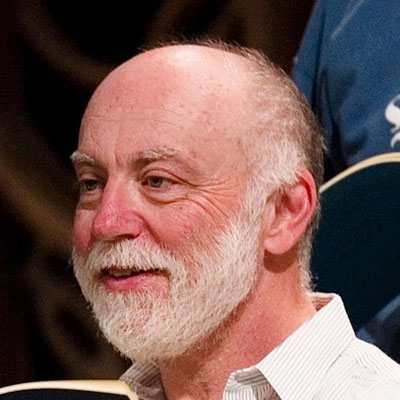
\includegraphics[width=4cm]{fig/deutsch.jpg}
      
      \textit{``To iterate is human, to recurse divine''}\\
      \small{
        \hfill L. Peter Deutsch (1946-)\\
               \hfill auteur de Ghostscript}
    }
  \end{columns}
  
\end{frame}

\begin{frame}[fragile]
\frametitle{Fonction r�cursive}
\begin{block}{}
Un algorithme r�cursif est un algorithme qui, lors
de son ex�cution, s'appelle lui-m�me.
\end{block}
\begin{exampleblock}{Algorithme factorielle}
\begin{algorithmic}[0]
\REQUIRE{n (entier)}\\
\ENSURE{nfact (entier)}\\
\IF {$n=0$}
\RETURN{1}
\ELSE
\RETURN {$n\times$factorielle$(n-1)$}
\ENDIF
\end{algorithmic}
\end{exampleblock}
Le langage C permet la r�cursivit� avec les fonctions :
\begin{codeblock}{}
\vspace{-.3cm}
\lstset{escapeinside={��}}
\lstset{basicstyle=\scriptsize}
\begin{codeC}
int fact (int n) {
  if (n==0) return (1) ;
  else return(n * fact (n-1));
}
\end{codeC}
\vspace{-.3cm}
\end{codeblock}
\end{frame}

\begin{frame}[fragile]
\frametitle{Contexte d'ex�cution}
\begin{block}{}
Chaque appel � la fonction cr�e son propre contexte d'ex�cution
(peut �tre gourmand en m�moire).
\end{block}
\begin{columns}
\column{0.5\textwidth}
\begin{codeblock}{}
\vspace{-.3cm}
\lstset{escapeinside={��}}
\lstset{basicstyle=\scriptsize}
\begin{codeC}
int fact (int n) {
  if (n==0) return (1) ;
  else return(n * fact (n-1));
}

int main() {
  int z ;
  z = fact(4);
}
\end{codeC}
\vspace{-.3cm}
\end{codeblock}

\column{0.4\textwidth}
\begin{figure}
\centering
\begin{tikzpicture}[
auto,
node distance=1cm,
]

\node (main) {main} ;
\node (f1) [below of = main] {fact} ;
\node (f2) [below of = f1] {fact} ;
\node (f3) [below of = f2] {fact} ;
\node (f4) [below of = f3] {fact} ;
\node (f5) [below of = f4] {fact} ;

\draw[->,thick] (main.220) -- node [midway, left] {4} (f1.140);
\draw[->,thick] (f1.220) -- node [midway, left] {3} (f2.140);
\draw[->,thick] (f2.220) -- node [midway, left] {2} (f3.140);
\draw[->,thick] (f3.220) -- node [midway, left] {1} (f4.140);
\draw[->,thick] (f4.220) -- node [midway, left] {0} (f5.140);

\draw[->,thick] (f5.40) -- node [midway, right] {1} (f4.320);
\draw[->,thick] (f4.40) -- node [midway, right] {1} (f3.320);
\draw[->,thick] (f3.40) -- node [midway, right] {2} (f2.320);
\draw[->,thick] (f2.40) -- node [midway, right] {6} (f1.320);
\draw[->,thick] (f1.40) -- node [midway, right] {24} (main.320);

\end{tikzpicture}
\end{figure}

\end{columns}

\end{frame}

\begin{frame}
\frametitle{Fonctions r�cursives}
\begin{block}{}
Selon les probl�me trait�s, la r�cursivit� permet
d'obtenir un code source succinct.
\end{block}
Par contre, quand elle est mal r�alis�e :
\begin{itemize}
\item Le code peut tourner sans fin ;
\item La m�moire utilis�e peut �tre �norme (� cause de
la multiplication des contextes d'ex�cution);
\item Cela peut ralentir l'ex�cution du programme.
\end{itemize}
\begin{alertblock}{}
A utiliser avec pr�caution.
\end{alertblock}
\end{frame}
% !TEX encoding = IsoLatin9

%%%%%%%%%%%%%%%%%%%%% SECTION 1
\section{Les fonctions standards}
\begin{frame}
  \begin{columns}
    \column{4.8cm}
    \tableofcontents[currentsection,hideothersubsections]
    \column{7cm}
    
  \end{columns}
  
\end{frame}

\begin{frame}[fragile]
\frametitle{La fonction \bvrb|rand|}
\begin{block}{Prototype}
\bvrb|int rand();|
\end{block}
\begin{itemize}
\setlength\itemsep{1em}
\item Renvoie un nombre al�atoire entre \Verb|0|
et \Verb|RAND_MAX|.
\item Utilisation :
\begin{columns}
\column{0.5\textwidth}
\begin{codeblock}{}
\vspace{-.3cm}
\lstset{escapeinside={��}}
\lstset{basicstyle=\scriptsize}
\begin{codeC}
#include <stdio.h>
#include <stdlib.h>

int main() {
  int alea ;
  alea = rand() ;
  printf("%d",alea);
}
\end{codeC}
\vspace{-.3cm}
\end{codeblock}
\column{0.4\textwidth}
Valeur type de \Verb|RAND_MAX| :
2~147~483~647
\end{columns}
\end{itemize}
\begin{alertblock}{}
Dans cet exemple, la valeur renvoy�e par \bvrb|rand|
sera la m�me � chaque ex�cution du programme
\end{alertblock}

\end{frame}

\begin{frame}[fragile]
\frametitle{Comment changer de nombre al�atoire � chaque ex�cution ?}
\begin{block}{La solution}
Il faut initialiser de mani�re diff�rente le g�n�rateur al�toire
� chaque ex�cution.\\
Astuce : Utiliser l'heure d'ex�cution.
\end{block}
\begin{codeblock}{}
\vspace{-.3cm}
\lstset{escapeinside={��}}
\lstset{basicstyle=\scriptsize}
\begin{codeC}
#include <stdio.h>
#include <stdlib.h>
#include <time.h>

int main() {
  int alea ;
  srand(time(NULL));
  alea = rand() ;
  printf("%d",alea);
}
\end{codeC}
\vspace{-.3cm}
\end{codeblock}
\end{frame}

\begin{frame}[fragile]
\frametitle{Les fonctions math�matiques \bvrb|math.h|}
\begin{codeblock}{}
\vspace{-.3cm}
\lstset{escapeinside={��}}
\lstset{basicstyle=\scriptsize}
\begin{codeC}
#include <math.h>
\end{codeC}
\vspace{-.3cm}
\end{codeblock}

\begin{figure}
\centering
\begin{tabular}{|c|c|c|c|c|c|}
\hline
\multicolumn{3}{|c|}{Donctions trigonom�triques} &
\multicolumn{3}{|c|}{Fonctions �l�mentaires} \\
\hline
\bvrb|sin(x)| & \bvrb|cos(x)| & \bvrb|tan(x)| &
\bvrb|exp(x)| & \bvrb|pow(x,y)| & \bvrb|sqrt(x)| \\
\hline
\bvrb|asin(x)| & \bvrb|acos(x)| & \bvrb|atan(x)| &
\bvrb|log(x)| & \bvrb|ceil(x)| & \bvrb|floor(x)| \\
\hline
\bvrb|sinh(x)| & \bvrb|cosh(x)| & \bvrb|tanh(x)| &
\bvrb|log10(x)| & \bvrb|fabs(x,y)| & \bvrb|fmod(x,y)| \\
\hline
\end{tabular}
\end{figure}

\begin{alertblock}{N�cessite l'option \bvrb|-lm| � la compilation}
\Verb|gcc -o prg prg.c -lm|
\end{alertblock}

\end{frame}
%% !TEX encoding = IsoLatin9

%%%%%%%%%%%%%%%%%%%%% SECTION 1
\section{Les cha�nes de caract�res}
\begin{frame}
  \begin{columns}
    \column{4.8cm}
    \tableofcontents[currentsection,hideothersubsections]
    \column{7cm}
    
  \end{columns}
  
\end{frame}

\begin{frame}[fragile]
\frametitle{Les cha�nes de caract�res}
\begin{itemize}
\setlength\itemsep{1em}
\item Les cha�nes de carat�res sont des tableaux
de caract�res ;
\item Chaque case du tableau contient un caract�re ;
\item Le dernier �l�ment est \red{toujours} \Verb|'\0'| ;
\item Pour socker une cha�ne de \Verb|n| �l�ments, il
faut \Verb|n+1| emplacements (� cause du \Verb|'\0'|).
\end{itemize}

\end{frame}

\begin{frame}[fragile]
\frametitle{Initialisation des cha�nes de carat�res}
\begin{block}{}
On peut utiliser les doubles quotes \Verb|"| pour initialiser
une cha�ne de caract�res.
\end{block}

\begin{codeblock}{}
\vspace{-.3cm}
\lstset{escapeinside={��}}
\lstset{basicstyle=\scriptsize}
\begin{codeC}
char tab[] = {'i','n','f','o','r','m','a','t','i','q','u','e','\0'};
\end{codeC}
\vspace{-.3cm}
\end{codeblock}
\vspace{1em}
\centering {ou}
\vspace{1em}
\begin{codeblock}{}
\vspace{-.3cm}
\lstset{escapeinside={��}}
\lstset{basicstyle=\scriptsize}
\begin{codeC}
char tab[] = "informatique";
\end{codeC}
\vspace{-.3cm}
\end{codeblock}
\end{frame}

\begin{frame}[fragile]
\frametitle{Le \bvrb|printf| et les cha�nes de caract�res}

\begin{block}{}
Le formateur de la cha�ne de caract�res dans le \bvrb|printf|
est \bvrb|%s|.
\end{block}
\vspace{1em}

Exemple :
\begin{codeblock}{}
\vspace{-.3cm}
\lstset{escapeinside={��}}
\lstset{basicstyle=\scriptsize}
\begin{codeC}
char tab[] = "informatique";
printf("Nous sommes en cours d'%s\n",tab);
\end{codeC}
\vspace{-.3cm}
\end{codeblock}
\end{frame}

\begin{frame}[fragile]
\frametitle{Saisie de cha�nes de carat�res au clavier}
Il existe deux fonctions en langage C permettant
de saisir des cha�nes de caract�res :
\begin{itemize}
\setlength\itemsep{1em}
\item \bvrb|scanf| (d�j� vu) ;
\item \bvrb|fgets| (sp�cifique pour les cha�nes de caract�res).
\end{itemize}
\end{frame}

\begin{frame}[fragile]
\frametitle{Les \bvrb|scanf| et les cha�nes de caract�res}
\begin{itemize}
\setlength\itemsep{1em}
\item Le formateur de la cha�ne de caract�re dans le
\bvrb|scanf| est \bvrb|%s|.
\item Pensez � d�clarer un tableau de caract�res d'une
taille suffisante avant de l'affecter dans le \bvrb|scanf|.
\item Il ne faut \red{pas} mettre le \bvrb|&|.
\end{itemize}
\begin{codeblock}{}
\vspace{-.3cm}
\lstset{escapeinside={��}}
%\lstset{basicstyle=\scriptsize}
\begin{codeC}
char nom[20];
printf("\n Entrez votre nom : ");
scanf("%s",nom);
printf("\n Bonjour %s !\n",nom);
\end{codeC}
\vspace{-.3cm}
\end{codeblock}

\end{frame}

\begin{frame}[fragile]
\frametitle{Rappel : le caract�re espace}

\begin{block}{}
Le caract�re espace est consid�r� comme un d�limiteur.
La conversion de la m�moire tampon en cha�ne de caract�res
s'arr�te donc � l'espace et ce dernier n'est pas consomm� :
il reste disponible pour la prochaine lecture.
\end{block}

\begin{columns}

\column{0.49\textwidth}

\begin{codeblock}{exemple.c}
\vspace{-.3cm}
\lstset{escapeinside={��}}
\lstset{basicstyle=\scriptsize}
\begin{codeC}
char nom[20];
printf("\n Entrez votre nom : ");
scanf("%s",nom);
printf("\n Bonjour %s !\n",nom);
\end{codeC}
\vspace{-.3cm}
\end{codeblock}

\column{0.45\textwidth}

\begin{termblock}{test 1}
\vspace{-.3cm}
\lstset{escapeinside={��}}
\lstset{basicstyle=\scriptsize}
\begin{lstlisting}
�\textbf{>>}�./exemple
�\color{darkgray}{\texttt{Entrez votre nom : }}� Dupont
�\color{darkgray}{\texttt{Bonjour Dupont ! }}�
\end{lstlisting}
\vspace{-.3cm}
\end{termblock}

\begin{termblock}{test 2}
\vspace{-.3cm}
\lstset{escapeinside={��}}
\lstset{basicstyle=\scriptsize}
\begin{lstlisting}
�\textbf{>>}�./exemple
�\color{darkgray}{\texttt{Entrez votre nom : }}� Dupont toto
�\color{darkgray}{\texttt{Bonjour Dupont ! }}�
\end{lstlisting}
\vspace{-.3cm}
\end{termblock}

\end{columns}
\begin{alertblock}{Conclusion}
Avec \bvrb|scanf| on ne peut pas saisir de cha�ne
de caract�res avec des espaces.
\end{alertblock}

\end{frame}

\begin{frame}[fragile]
\frametitle{Autre solution : \bvrb|fgets|}
\centering{
  \bvrb|fgets(�textit�string�,�textit�taille�,stdin);|
}
\begin{columns}

\column{0.49\textwidth}

\begin{codeblock}{exemple.c}
\vspace{-.3cm}
\lstset{escapeinside={��}}
\lstset{basicstyle=\scriptsize}
\begin{codeC}
char nom[20];
printf("\n Entrez votre nom : ");
fgets (nom,19,stdin) ;
printf("\n Bonjour %s !\n",nom);
\end{codeC}
\vspace{-.3cm}
\end{codeblock}

\column{0.45\textwidth}

\begin{termblock}{test}
\vspace{-.3cm}
\lstset{escapeinside={��}}
\lstset{basicstyle=\scriptsize}
\begin{lstlisting}
�\textbf{>>}�./exemple
�\color{darkgray}{\texttt{Entrez votre nom : }}� Dupont toto
�\color{darkgray}{\texttt{Bonjour Dupont toto ! }}�
\end{lstlisting}
\vspace{-.3cm}
\end{termblock}
\end{columns}

\begin{itemize}
\item Avec \bvrb|fgets|, seule la fin de ligne sert de d�limiteur.
\item \bvrb|�textit�taille�| est le nombre maximum de caract�res
qui peuvent �tre lus.
\item \bvrb|stdin| indique qu'on doit lire les caract�res
dans "l'entr�e standard", c'est � dire dans ce que vous tapez
au clavier. On peut aussi lire les caract�res dans un fichier
(cf cours n$^o$ 7)
\item \red{ATTENTION} : la cha�ne de caract�re lue contiendra le
retour � la ligne.
Dans l'exemple pr�c�dent 
\Verb|nom='D','u','p','o','n','t',' ','t','o','t','o','\n','\0'|
\end{itemize}

\end{frame}

\begin{frame}
\frametitle{�galit� de cha�nes de caract�res}
\begin{block}{}
Pour v�rifier l'�galit� de deux cha�nes de caract�res,
il faut v�rifier un par un tous les caract�res (comme
pour un autre tableau).
\end{block}

\vspace{1em}
\begin{exampleblock}{Exemple :}

Demander � l'utilisateur d'entrer \Verb|pluie| ou \Verb|soleil|,
et afficher "Prenez un parapluie" si l'utilisateur � mis pluie.
\end{exampleblock}
\end{frame}

\begin{frame}[fragile]
\frametitle{La biblioth�que \bvrb|string.h|}
\begin{codeblock}{exemple.c}
\vspace{-.3cm}
\lstset{escapeinside={��}}
%\lstset{basicstyle=\scriptsize}
\begin{codeC}
#include <string.h>
\end{codeC}
\vspace{-.3cm}
\end{codeblock}

\begin{block}{}
Contient des fonctions standards pour g�rer les 
cha�nes de caract�res
\end{block}
Exemples :
\begin{figure}
\centering
\begin{tabular}{|c|p{3.8cm}|}
\hline
Prototype de la fonction & Utilisation \\
\hline
\bvrb|int strcmp(char �textit�s1�[], char �textit�s2�[]);| &
\red{Renvoie}  si les les cha�nes \bvrb|�textit�s1�| et \bvrb|�textit�s2�|
sont �gales.\\
\hline
\bvrb|int strlen(char �textit�s�[]);| & 
Renvoie la taille de \bvrb|�textit�s�|\\
\hline
\end{tabular}
\end{figure}

Pour le d�tail de toutes les fonctions :
\begin{termblock}{}
\vspace{-.3cm}
\lstset{escapeinside={��}}
%\lstset{basicstyle=\scriptsize}
\begin{lstlisting}
�\textbf{>>}� man string
\end{lstlisting}
\vspace{-.3cm}
\end{termblock}
\end{frame}
\end{document} 

%%%%%%%%%%%%%%%%%%%%% SECTION 1
\section{Les algorithmes}\label{section:1}
\begin{frame}
\begin{columns}
        \column{4.8cm}
            \tableofcontents[currentsection]
        \column{7cm}
        \centering{
            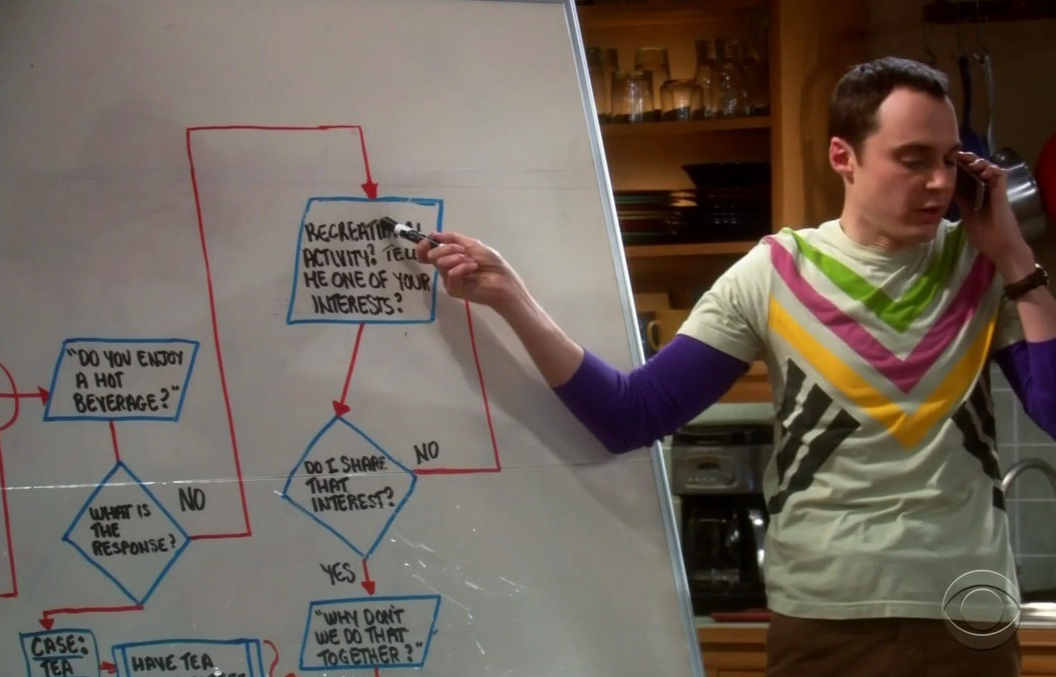
\includegraphics[width=7cm]{fig/Algorithm-sheldon.png}
            
                 \textit{ I believe I've isolateblblblblblblsblbslbslbsl
            sblbslblsblsblblsblbs
            lbslblbslsb d the algorithm for making friends.}
     
            
            \small{
            \hfill Sheldon Cooper, 
            
            \hfill in \textit{The Big Band Theory}, Season 2, Episode 13
            }
}

    \end{columns}

\end{frame}


%%%%%%%%%%%%%%%%%%%%%
\subsection{Introduction}
    \begin{frame}
    \frametitle{Pourquoi faire appel � des algorithmes ?}
    Pour automatiser des t�ches
    
    Exemples :
    \begin{itemize}
    \item M�tier � tisser\\
    \item M�thode de calcul � la main d'une division\\
    \item Recette de cuisine\\
    \item ...\\
    \end{itemize}
    \end{frame}
 
 %%%%%%%%%%%%%%%%%
 
    \begin{frame}
    \frametitle{Qu'est-ce qu'un algorithme ?}
    \begin{block}{D�finition}
    Un algorithme est un ensemble 
    ordonn� d'instructions simples
permettant de r�soudre un probl�me.
    \end{block}
    \end{frame}
    
 %%%%%%%%%%%%%%%%%%
 \subsection{Construction d'un algorithme}
%%%%%%%%%%%%%%%%%%%    
\section{La machine de Turing}
%%%%%%%%%%%%%%%%%%%%
 
  
\begin{frame}[fragile]
\frametitle{Un peu d'histoire...}
\begin{codeblock}{Test}
\begin{codeC}
for (int i = 0 ; i < n ; i ++) {
    //a comment
    printf("%d",i);
    }
\end{codeC}
\end{codeblock}

\begin{termblock}{test 2}
\lstset{escapeinside={��}}
\begin{lstlisting}
�\textbf{>>}�./a.out
�\color{darkgray}{\texttt{  Hello World}}�
\end{lstlisting}
\end{termblock}

 \begin{block}{Bloc standard}
blablabla
\end{block}
\end{frame}


\begin{frame}[fragile]
\frametitle{essai}
\begin{columns}
\column{6cm}
\begin{block}

\begin{figure}
\begin{tikzpicture} [
    auto,
    decision/.style = { diamond, draw=blue, thick, fill=blue!20,
                        text width=5em, text badly centered,
                        inner sep=1pt, rounded corners },
    block/.style    = { rectangle, draw=blue, thick, 
                        fill=blue!20, text width=10em, text centered,
                        rounded corners, minimum height=2em },
    line/.style     = { draw, thick, ->, shorten >=2pt },
  ]
   \matrix [column sep=-10mm, row sep=10mm] {
                    & \node [text centered] (x) {$\mathbf{X}$};            & \\
                    & \node (null1) {};                                    & \\
                    & \node [block] (doa) {\textsf{DoAE}($\mathbf{X}$)};   & \\
  	               \node(null3){}; & \node [decision] (uiddes)
                        {\textsf{UID}($\hat{\mathbf{X}}$)};
                                  & \node[text centered](tra){$\mathbf{i}$}; \\
                  & \node [block] (track) {\textsf{DoAT}($\mathbf{x}$)}; & \\
                    & \node [block] (pesos)
                        {\textsf{BF}(DoA$_{\mathrm{T}}$,DoAs)};            & \\
                    & \node [block] (filtrado)
                        {\textsf{SF}($\mathbf{w}$,$\mathbf{x}$)};          & \\
                    & \node [text centered] (xf) {$\hat{x}(t)$ };          & \\
  };
  % connect all nodes defined above
 \begin{scope} [every path/.style=line]
    \path (x)        --    (doa);
    \path (doa)      --    node [near start] {DoAs} (uiddes);
    \path (tra)      --    (uiddes);
    \path (uiddes)   --++  (-3,0) node [near start] {no} |- (null1);
    \path (uiddes)   --    node [near start] {DoA} (track);
    \path (track)    --    node [near start] {DoA$_{\mathrm{T}}$} (pesos);
    \path (pesos)    --    node [near start] {\textbf{w}} (filtrado);
    \path (filtrado) --    (xf);
  
  \end{scope}
\end{tikzpicture}
\end{figure}
\end{block}
\column{3cm}
\begin{block}{bulbul}
\end{block}
\end{columns}
\end{frame}

\end{document}
